% Created by tikzDevice version 0.12.6 on 2024-04-10 20:49:09
% !TEX encoding = UTF-8 Unicode
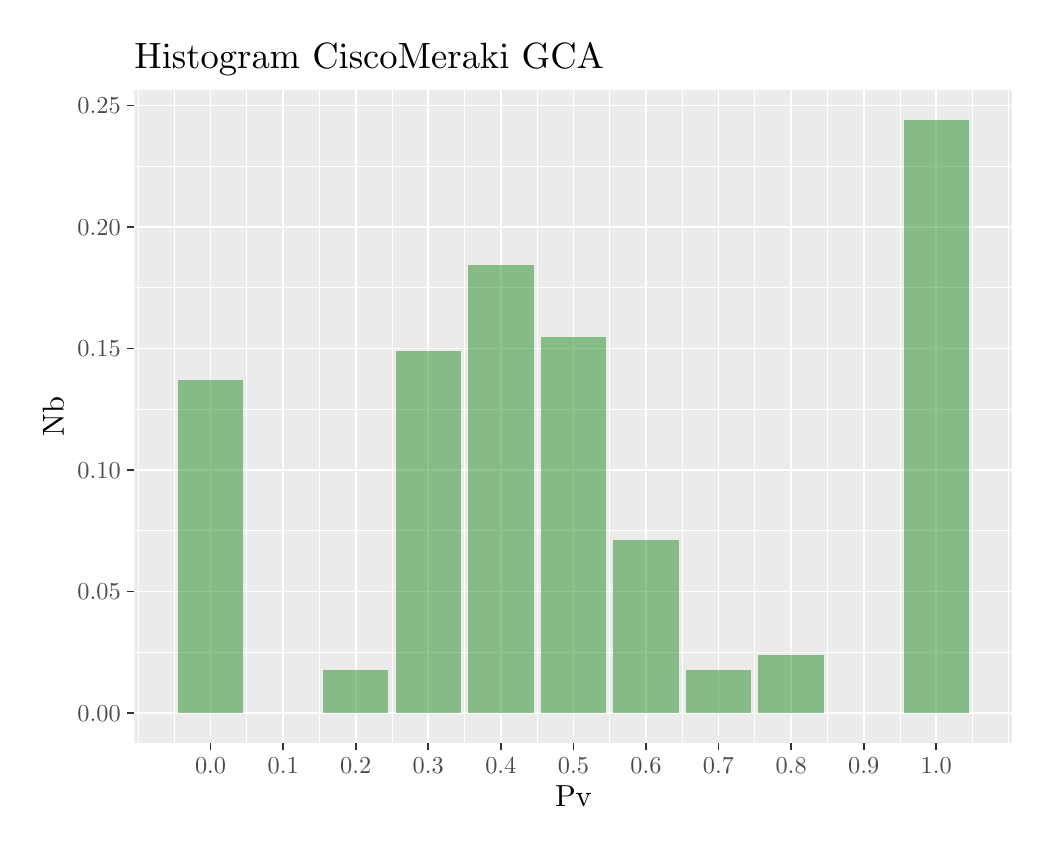
\begin{tikzpicture}[x=1pt,y=1pt]
\definecolor{fillColor}{RGB}{255,255,255}
\path[use as bounding box,fill=fillColor,fill opacity=0.00] (0,0) rectangle (361.35,289.08);
\begin{scope}
\path[clip] (  0.00,  0.00) rectangle (361.35,289.08);
\definecolor{drawColor}{RGB}{255,255,255}
\definecolor{fillColor}{RGB}{255,255,255}

\path[draw=drawColor,line width= 0.6pt,line join=round,line cap=round,fill=fillColor] (  0.00,  0.00) rectangle (361.35,289.08);
\end{scope}
\begin{scope}
\path[clip] ( 38.56, 30.69) rectangle (355.85,266.42);
\definecolor{fillColor}{gray}{0.92}

\path[fill=fillColor] ( 38.56, 30.69) rectangle (355.85,266.42);
\definecolor{drawColor}{RGB}{255,255,255}

\path[draw=drawColor,line width= 0.3pt,line join=round] ( 38.56, 63.35) --
	(355.85, 63.35);

\path[draw=drawColor,line width= 0.3pt,line join=round] ( 38.56,107.26) --
	(355.85,107.26);

\path[draw=drawColor,line width= 0.3pt,line join=round] ( 38.56,151.17) --
	(355.85,151.17);

\path[draw=drawColor,line width= 0.3pt,line join=round] ( 38.56,195.07) --
	(355.85,195.07);

\path[draw=drawColor,line width= 0.3pt,line join=round] ( 38.56,238.98) --
	(355.85,238.98);

\path[draw=drawColor,line width= 0.3pt,line join=round] ( 39.87, 30.69) --
	( 39.87,266.42);

\path[draw=drawColor,line width= 0.3pt,line join=round] ( 52.98, 30.69) --
	( 52.98,266.42);

\path[draw=drawColor,line width= 0.3pt,line join=round] ( 79.20, 30.69) --
	( 79.20,266.42);

\path[draw=drawColor,line width= 0.3pt,line join=round] (105.42, 30.69) --
	(105.42,266.42);

\path[draw=drawColor,line width= 0.3pt,line join=round] (131.65, 30.69) --
	(131.65,266.42);

\path[draw=drawColor,line width= 0.3pt,line join=round] (157.87, 30.69) --
	(157.87,266.42);

\path[draw=drawColor,line width= 0.3pt,line join=round] (184.09, 30.69) --
	(184.09,266.42);

\path[draw=drawColor,line width= 0.3pt,line join=round] (210.31, 30.69) --
	(210.31,266.42);

\path[draw=drawColor,line width= 0.3pt,line join=round] (236.54, 30.69) --
	(236.54,266.42);

\path[draw=drawColor,line width= 0.3pt,line join=round] (262.76, 30.69) --
	(262.76,266.42);

\path[draw=drawColor,line width= 0.3pt,line join=round] (288.98, 30.69) --
	(288.98,266.42);

\path[draw=drawColor,line width= 0.3pt,line join=round] (315.20, 30.69) --
	(315.20,266.42);

\path[draw=drawColor,line width= 0.3pt,line join=round] (341.43, 30.69) --
	(341.43,266.42);

\path[draw=drawColor,line width= 0.3pt,line join=round] (354.54, 30.69) --
	(354.54,266.42);

\path[draw=drawColor,line width= 0.6pt,line join=round] ( 38.56, 41.40) --
	(355.85, 41.40);

\path[draw=drawColor,line width= 0.6pt,line join=round] ( 38.56, 85.31) --
	(355.85, 85.31);

\path[draw=drawColor,line width= 0.6pt,line join=round] ( 38.56,129.21) --
	(355.85,129.21);

\path[draw=drawColor,line width= 0.6pt,line join=round] ( 38.56,173.12) --
	(355.85,173.12);

\path[draw=drawColor,line width= 0.6pt,line join=round] ( 38.56,217.03) --
	(355.85,217.03);

\path[draw=drawColor,line width= 0.6pt,line join=round] ( 38.56,260.93) --
	(355.85,260.93);

\path[draw=drawColor,line width= 0.6pt,line join=round] ( 66.09, 30.69) --
	( 66.09,266.42);

\path[draw=drawColor,line width= 0.6pt,line join=round] ( 92.31, 30.69) --
	( 92.31,266.42);

\path[draw=drawColor,line width= 0.6pt,line join=round] (118.53, 30.69) --
	(118.53,266.42);

\path[draw=drawColor,line width= 0.6pt,line join=round] (144.76, 30.69) --
	(144.76,266.42);

\path[draw=drawColor,line width= 0.6pt,line join=round] (170.98, 30.69) --
	(170.98,266.42);

\path[draw=drawColor,line width= 0.6pt,line join=round] (197.20, 30.69) --
	(197.20,266.42);

\path[draw=drawColor,line width= 0.6pt,line join=round] (223.43, 30.69) --
	(223.43,266.42);

\path[draw=drawColor,line width= 0.6pt,line join=round] (249.65, 30.69) --
	(249.65,266.42);

\path[draw=drawColor,line width= 0.6pt,line join=round] (275.87, 30.69) --
	(275.87,266.42);

\path[draw=drawColor,line width= 0.6pt,line join=round] (302.09, 30.69) --
	(302.09,266.42);

\path[draw=drawColor,line width= 0.6pt,line join=round] (328.32, 30.69) --
	(328.32,266.42);
\definecolor{fillColor}{RGB}{34,139,34}

\path[fill=fillColor,fill opacity=0.50] ( 54.29, 41.40) rectangle ( 77.89,161.62);

\path[fill=fillColor,fill opacity=0.50] (106.73, 41.40) rectangle (130.33, 57.08);

\path[fill=fillColor,fill opacity=0.50] (132.96, 41.40) rectangle (156.56,172.08);

\path[fill=fillColor,fill opacity=0.50] (159.18, 41.40) rectangle (182.78,203.44);

\path[fill=fillColor,fill opacity=0.50] (185.40, 41.40) rectangle (209.00,177.30);

\path[fill=fillColor,fill opacity=0.50] (211.63, 41.40) rectangle (235.23,104.12);

\path[fill=fillColor,fill opacity=0.50] (237.85, 41.40) rectangle (261.45, 57.08);

\path[fill=fillColor,fill opacity=0.50] (264.07, 41.40) rectangle (287.67, 62.31);

\path[fill=fillColor,fill opacity=0.50] (316.52, 41.40) rectangle (340.12,255.71);
\end{scope}
\begin{scope}
\path[clip] (  0.00,  0.00) rectangle (361.35,289.08);
\definecolor{drawColor}{gray}{0.30}

\node[text=drawColor,anchor=base east,inner sep=0pt, outer sep=0pt, scale=  0.88] at ( 33.61, 38.37) {0.00};

\node[text=drawColor,anchor=base east,inner sep=0pt, outer sep=0pt, scale=  0.88] at ( 33.61, 82.28) {0.05};

\node[text=drawColor,anchor=base east,inner sep=0pt, outer sep=0pt, scale=  0.88] at ( 33.61,126.18) {0.10};

\node[text=drawColor,anchor=base east,inner sep=0pt, outer sep=0pt, scale=  0.88] at ( 33.61,170.09) {0.15};

\node[text=drawColor,anchor=base east,inner sep=0pt, outer sep=0pt, scale=  0.88] at ( 33.61,214.00) {0.20};

\node[text=drawColor,anchor=base east,inner sep=0pt, outer sep=0pt, scale=  0.88] at ( 33.61,257.90) {0.25};
\end{scope}
\begin{scope}
\path[clip] (  0.00,  0.00) rectangle (361.35,289.08);
\definecolor{drawColor}{gray}{0.20}

\path[draw=drawColor,line width= 0.6pt,line join=round] ( 35.81, 41.40) --
	( 38.56, 41.40);

\path[draw=drawColor,line width= 0.6pt,line join=round] ( 35.81, 85.31) --
	( 38.56, 85.31);

\path[draw=drawColor,line width= 0.6pt,line join=round] ( 35.81,129.21) --
	( 38.56,129.21);

\path[draw=drawColor,line width= 0.6pt,line join=round] ( 35.81,173.12) --
	( 38.56,173.12);

\path[draw=drawColor,line width= 0.6pt,line join=round] ( 35.81,217.03) --
	( 38.56,217.03);

\path[draw=drawColor,line width= 0.6pt,line join=round] ( 35.81,260.93) --
	( 38.56,260.93);
\end{scope}
\begin{scope}
\path[clip] (  0.00,  0.00) rectangle (361.35,289.08);
\definecolor{drawColor}{gray}{0.20}

\path[draw=drawColor,line width= 0.6pt,line join=round] ( 66.09, 27.94) --
	( 66.09, 30.69);

\path[draw=drawColor,line width= 0.6pt,line join=round] ( 92.31, 27.94) --
	( 92.31, 30.69);

\path[draw=drawColor,line width= 0.6pt,line join=round] (118.53, 27.94) --
	(118.53, 30.69);

\path[draw=drawColor,line width= 0.6pt,line join=round] (144.76, 27.94) --
	(144.76, 30.69);

\path[draw=drawColor,line width= 0.6pt,line join=round] (170.98, 27.94) --
	(170.98, 30.69);

\path[draw=drawColor,line width= 0.6pt,line join=round] (197.20, 27.94) --
	(197.20, 30.69);

\path[draw=drawColor,line width= 0.6pt,line join=round] (223.43, 27.94) --
	(223.43, 30.69);

\path[draw=drawColor,line width= 0.6pt,line join=round] (249.65, 27.94) --
	(249.65, 30.69);

\path[draw=drawColor,line width= 0.6pt,line join=round] (275.87, 27.94) --
	(275.87, 30.69);

\path[draw=drawColor,line width= 0.6pt,line join=round] (302.09, 27.94) --
	(302.09, 30.69);

\path[draw=drawColor,line width= 0.6pt,line join=round] (328.32, 27.94) --
	(328.32, 30.69);
\end{scope}
\begin{scope}
\path[clip] (  0.00,  0.00) rectangle (361.35,289.08);
\definecolor{drawColor}{gray}{0.30}

\node[text=drawColor,anchor=base,inner sep=0pt, outer sep=0pt, scale=  0.88] at ( 66.09, 19.68) {0.0};

\node[text=drawColor,anchor=base,inner sep=0pt, outer sep=0pt, scale=  0.88] at ( 92.31, 19.68) {0.1};

\node[text=drawColor,anchor=base,inner sep=0pt, outer sep=0pt, scale=  0.88] at (118.53, 19.68) {0.2};

\node[text=drawColor,anchor=base,inner sep=0pt, outer sep=0pt, scale=  0.88] at (144.76, 19.68) {0.3};

\node[text=drawColor,anchor=base,inner sep=0pt, outer sep=0pt, scale=  0.88] at (170.98, 19.68) {0.4};

\node[text=drawColor,anchor=base,inner sep=0pt, outer sep=0pt, scale=  0.88] at (197.20, 19.68) {0.5};

\node[text=drawColor,anchor=base,inner sep=0pt, outer sep=0pt, scale=  0.88] at (223.43, 19.68) {0.6};

\node[text=drawColor,anchor=base,inner sep=0pt, outer sep=0pt, scale=  0.88] at (249.65, 19.68) {0.7};

\node[text=drawColor,anchor=base,inner sep=0pt, outer sep=0pt, scale=  0.88] at (275.87, 19.68) {0.8};

\node[text=drawColor,anchor=base,inner sep=0pt, outer sep=0pt, scale=  0.88] at (302.09, 19.68) {0.9};

\node[text=drawColor,anchor=base,inner sep=0pt, outer sep=0pt, scale=  0.88] at (328.32, 19.68) {1.0};
\end{scope}
\begin{scope}
\path[clip] (  0.00,  0.00) rectangle (361.35,289.08);
\definecolor{drawColor}{RGB}{0,0,0}

\node[text=drawColor,anchor=base,inner sep=0pt, outer sep=0pt, scale=  1.10] at (197.20,  7.64) {Pv};
\end{scope}
\begin{scope}
\path[clip] (  0.00,  0.00) rectangle (361.35,289.08);
\definecolor{drawColor}{RGB}{0,0,0}

\node[text=drawColor,rotate= 90.00,anchor=base,inner sep=0pt, outer sep=0pt, scale=  1.10] at ( 13.08,148.55) {Nb};
\end{scope}
\begin{scope}
\path[clip] (  0.00,  0.00) rectangle (361.35,289.08);
\definecolor{drawColor}{RGB}{0,0,0}

\node[text=drawColor,anchor=base west,inner sep=0pt, outer sep=0pt, scale=  1.32] at ( 38.56,274.49) {Histogram CiscoMeraki GCA};
\end{scope}
\end{tikzpicture}
